\documentclass[aspectratio=169,10pt]{beamer}

\usepackage[T1]{fontenc}
\usepackage[utf8]{inputenc}
\usepackage{amsmath}
\usepackage{array}
\usepackage{booktabs}
\usepackage{graphicx}
\usepackage{ragged2e}
\usepackage{tabularx}
\usepackage{tikz}
\usetikzlibrary{arrows.meta,positioning,shapes.geometric}

\graphicspath{
  {artifacts/tcga/report/}
  {artifacts/tcga/classification/}
  {artifacts/tcga/clustering/}
  {artifacts/tcga/pca_covariance/}
}

\definecolor{DeckGreen}{HTML}{173F35}
\definecolor{DeckBlue}{HTML}{163A5F}
\definecolor{DeckGold}{HTML}{B4852B}
\definecolor{DeckClay}{HTML}{A85D43}
\definecolor{DeckInk}{HTML}{1F2A35}
\definecolor{DeckSoft}{HTML}{4C5964}
\definecolor{DeckPaper}{HTML}{FAF8F2}
\definecolor{DeckMist}{HTML}{E2E7E3}
\definecolor{DeckSilver}{HTML}{A4AFB7}

\setbeamertemplate{navigation symbols}{}
\setbeamertemplate{blocks}[rounded][shadow=false]

\setbeamercolor{normal text}{fg=DeckInk,bg=DeckPaper}
\setbeamercolor{structure}{fg=DeckGreen}
\setbeamercolor{frametitle}{fg=DeckInk,bg=DeckPaper}
\setbeamercolor{title}{fg=DeckInk}
\setbeamercolor{subtitle}{fg=DeckSoft}
\setbeamercolor{author}{fg=DeckSoft}
\setbeamercolor{date}{fg=DeckSoft}
\setbeamercolor{block title}{fg=white,bg=DeckGreen}
\setbeamercolor{block body}{fg=DeckInk,bg=white}
\setbeamercolor{alerted text}{fg=DeckClay}
\setbeamercolor{item}{fg=DeckGreen}

\setbeamerfont{title}{series=\bfseries,size=\LARGE}
\setbeamerfont{subtitle}{size=\large}
\setbeamerfont{frametitle}{series=\bfseries,size=\Large}
\setbeamerfont{block title}{series=\bfseries}

\setbeamertemplate{frametitle}{
  \vspace{0.15cm}
  \begin{beamercolorbox}[wd=\paperwidth,leftskip=0.7cm,rightskip=0.35cm,ht=0.95cm,dp=0.22cm]{frametitle}
    \usebeamerfont{frametitle}\insertframetitle
  \end{beamercolorbox}
}

\setbeamertemplate{footline}{
  \leavevmode
  \hbox{
    \begin{beamercolorbox}[wd=.78\paperwidth,ht=0.34cm,dp=0.12cm]{author in head/foot}
      \hspace*{0.35cm}%
      \color{DeckSoft}\scriptsize STAT 662 | TCGA Pan-Cancer Transcriptomic Analysis
    \end{beamercolorbox}
    \begin{beamercolorbox}[wd=.22\paperwidth,ht=0.34cm,dp=0.12cm,right]{date in head/foot}
      \color{DeckSoft}\scriptsize \insertframenumber{} / \inserttotalframenumber\hspace*{0.35cm}
    \end{beamercolorbox}
  }
}

\setbeamertemplate{itemize item}{\raise0.15ex\hbox{\small\color{DeckGreen}$\blacktriangleright$}}
\setbeamertemplate{itemize subitem}{\raise0.15ex\hbox{\scriptsize\color{DeckGold}$\bullet$}}

\newcommand{\tcga}{TCGA PanCanAtlas}
\newcommand{\bestclf}{Logistic Regression}
\newcommand{\bestcluster}{K-means}

\newcommand{\statcard}[2]{%
  \begin{beamercolorbox}[wd=\linewidth,sep=0.7ex,rounded=true]{block body}
    {\centering\color{DeckGreen}\bfseries\Large #1\par}
    \vspace{0.2em}
    {\centering\color{DeckSoft}\footnotesize #2\par}
  \end{beamercolorbox}
}

\title{Integrated Multivariate Analysis of \tcga\ Transcriptomic Data}
\subtitle{STAT 662 Final Presentation}
\author{Amandeep Singh}
\date{May 11, 2026}

\begin{document}

\begin{frame}[plain]
  \vspace{0.5cm}
  {\usebeamerfont{title}\color{DeckInk}\inserttitle\par}
  \vspace{0.25cm}
  {\usebeamerfont{subtitle}\color{DeckSoft}\insertsubtitle\par}
  \vspace{0.55cm}
  \begin{block}{Study question}
    \justifying
    Can high-dimensional pan-cancer RNA-seq profiles be compressed into stable latent structure that is clinically meaningful, predictive of cancer type, and informative for unsupervised tumor grouping?
  \end{block}
  \vspace{0.2cm}
  \begin{columns}[T,onlytextwidth]
    \column{0.24\textwidth}
      \statcard{10,055}{Representative tumor samples}
    \column{0.24\textwidth}
      \statcard{32}{Cancer types}
    \column{0.24\textwidth}
      \statcard{0.893}{Best held-out macro-F1}
    \column{0.24\textwidth}
      \statcard{0.541}{Best clustering ARI}
  \end{columns}
  \vfill
  {\color{DeckSoft}\small George Mason University \hfill Amandeep Singh \hfill May 11, 2026\par}
\end{frame}

\begin{frame}{Research Problem}
  \begin{columns}[T,onlytextwidth]
    \column{0.50\textwidth}
      \begin{block}{Why this is a challenging statistical problem}
        \small
        \begin{itemize}
          \item Each sample starts with \alert{20,531 gene-expression variables}.
          \item Gene measurements are highly correlated and biologically structured.
          \item The cohort spans \alert{32 cancer types} with uneven class sizes.
          \item Some cancers have overlapping transcriptomic programs, making prediction and clustering nontrivial.
        \end{itemize}
      \end{block}
    \column{0.47\textwidth}
      \begin{block}{Study objectives}
        \small
        \begin{enumerate}
          \item Summarize dominant transcriptomic variation with PCA.
          \item Quantify how age, sex, stage, and cancer type explain latent expression scores.
          \item Predict cancer type from a shared low-dimensional expression representation.
          \item Test whether unlabeled tumors recover known structure through clustering.
        \end{enumerate}
      \end{block}
    \end{columns}
    \vspace{0.1cm}
    {\small\color{DeckSoft}One integrated pipeline links molecular structure, clinical association, prediction, and unsupervised recovery from the same transcriptomic signal.\par}
\end{frame}

\begin{frame}{Data and Cohort Construction}
  \begin{columns}[T,onlytextwidth]
    \column{0.42\textwidth}
      \begin{block}{Cohort design}
        \small
        \begin{itemize}
          \item Parse each TCGA barcode to recover patient identity and sample type.
          \item Keep tumor-derived specimens only.
          \item Select one \alert{representative sample per patient}, prioritizing primary solid tumor.
          \item Harmonize with clinical covariates and clean the expression matrix.
        \end{itemize}
      \end{block}
    \column{0.55\textwidth}
      \includegraphics[height=0.57\textheight]{report_cancer_counts.pdf}
      {\scriptsize\color{DeckSoft}Largest cohorts: BRCA 1,097; KIRC 533; UCEC 532; HNSC 520; LUAD 515.\par}
    \end{columns}
    \vspace{0.08cm}
    {\small\color{DeckSoft}11,069 manifest rows | 10,274 patients | 10,055 final cohort | 8,044 / 2,011 train / test.\par}
\end{frame}

\begin{frame}{Analysis Workflow}
  \centering
  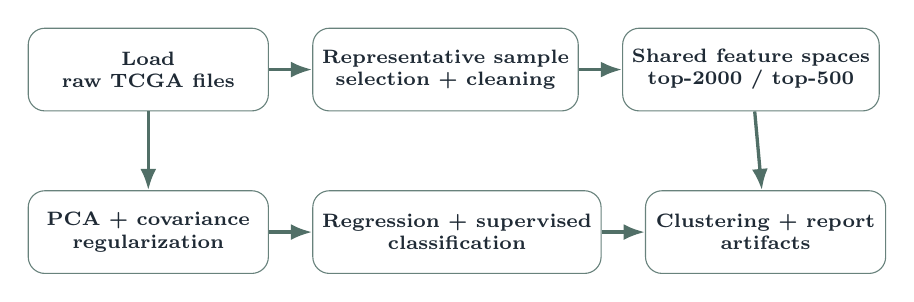
\begin{tikzpicture}[
    node distance=0.55cm,
    box/.style={
      rounded corners=6pt,
      draw=DeckGreen!65,
      fill=white,
      minimum width=3.05cm,
      minimum height=1.05cm,
      align=center,
      text=DeckInk,
      font=\scriptsize\bfseries
    },
    arrow/.style={-{Latex[length=2.7mm]}, very thick, draw=DeckGreen!75}
  ]
    \node[box] (load) {Load\\raw TCGA files};
    \node[box, right=of load] (prep) {Representative sample\\selection + cleaning};
    \node[box, right=of prep] (feat) {Shared feature spaces\\top-2000 / top-500};

    \node[box, below=1.0cm of load] (pca) {PCA + covariance\\regularization};
    \node[box, right=of pca] (sup) {Regression + supervised\\classification};
    \node[box, right=of sup] (unsup) {Clustering + report\\artifacts};

    \draw[arrow] (load) -- (prep);
    \draw[arrow] (prep) -- (feat);
    \draw[arrow] (feat) -- (unsup);
    \draw[arrow] (load) -- (pca);
    \draw[arrow] (pca) -- (sup);
    \draw[arrow] (sup) -- (unsup);
  \end{tikzpicture}

  \vspace{0.35cm}
  \begin{block}{Evaluation settings}
    \small
    Classification uses a stratified 80/20 split with 5-fold CV; PCA stability uses 10 repeated 80\% subsamples; clustering stability is measured by repeated-subsample ARI.
  \end{block}
\end{frame}

\begin{frame}{PCA and Covariance Results}
  \begin{columns}[T,onlytextwidth]
    \column{0.56\textwidth}
      \includegraphics[width=\linewidth]{top15_pc_explained_variance.pdf}
    \column{0.40\textwidth}
      \begin{block}{Dimensionality}
        \small
        \begin{itemize}
          \item PC1 variance: \alert{6.61\%}
          \item First 10 PCs: \alert{34.35\%}
          \item First 50 PCs: \alert{57.94\%}
        \end{itemize}
      \end{block}
      \begin{block}{Stability and covariance}
        \footnotesize
        \begin{itemize}
          \item PCs 1--5 loading correlation: \alert{$> 0.997$}
          \item Mean subspace similarity: \alert{0.9995}
          \item Graphical Lasso penalty: \alert{0.5543}
        \end{itemize}
      \end{block}
  \end{columns}
\end{frame}

\begin{frame}{Multivariate Regression on Latent Expression Scores}
  \begin{columns}[T,onlytextwidth]
    \column{0.56\textwidth}
      \includegraphics[width=\linewidth]{regression_block_cv_delta_r2.pdf}
    \column{0.41\textwidth}
      \begin{block}{Key regression findings}
        \footnotesize
        \begin{itemize}
          \item Response: first 10 PC scores; predictors: age, sex, stage, and cancer acronym.
          \item Multivariate ridge with 5-fold CV gives variance-weighted $R^2 = \alert{0.6944}$.
          \item Overall permutation significance remains detectable: $p = \alert{0.0385}$.
          \item Cancer acronym is dominant (delta-$R^2 = \alert{0.5561}$); stage is modest; age and sex are negligible after conditioning on cancer type.
        \end{itemize}
      \end{block}
    \end{columns}
\end{frame}

\begin{frame}{Supervised Cancer-Type Prediction: Experimental Setup}
  \begin{columns}[T,onlytextwidth]
    \column{0.50\textwidth}
      \begin{block}{Representation}
        \small
        \begin{itemize}
          \item Shared top-2,000 gene matrix
          \item Train-only standardization
          \item PCA embedding with \alert{50 PCs}
        \end{itemize}
      \end{block}
      \begin{block}{Models compared}
        \footnotesize
        Logistic Regression, Linear SVM, RBF SVM, Random Forest, Histogram Gradient Boosting, and Multilayer Perceptron.
      \end{block}
    \column{0.47\textwidth}
      \begin{block}{Validation protocol}
        \footnotesize
        \begin{itemize}
          \item Stratified 80/20 split
          \item Training rows: \alert{8,044}
          \item Test rows: \alert{2,011}
          \item Hyperparameter tuning: \alert{5-fold CV}
          \item Selection metric: \alert{macro-F1}
        \end{itemize}
      \end{block}
      {\footnotesize\color{DeckSoft}Macro-F1 emphasizes balanced performance across all 32 cancers rather than letting the largest classes dominate the score.\par}
    \end{columns}
\end{frame}

\begin{frame}{Supervised Classification Results}
  \begin{columns}[T,onlytextwidth]
    \column{0.58\textwidth}
      \includegraphics[width=\linewidth]{classification_model_comparison.pdf}
    \column{0.39\textwidth}
      \begin{block}{Best overall model}
        \small
        \bestclf
        \begin{itemize}
          \item Accuracy: \alert{0.9115}
          \item Macro-F1: \alert{0.8928}
          \item Weighted F1: \alert{0.9141}
          \item Best CV macro-F1: \alert{0.8727}
        \end{itemize}
      \end{block}
      \begin{block}{Important comparison}
        \small
        MLP has slightly higher raw accuracy (\alert{0.9135}) but lower macro-F1 (\alert{0.8809}), so Logistic Regression is the strongest balanced model.
      \end{block}
    \end{columns}
\end{frame}

\begin{frame}{Classification Diagnostics}
  \begin{columns}[T,onlytextwidth]
    \column{0.58\textwidth}
      \includegraphics[height=0.69\textheight,keepaspectratio]{best_classifier_per_class_f1.pdf}
    \column{0.38\textwidth}
      \begin{block}{Class-level performance}
        \footnotesize
        \begin{itemize}
          \item \alert{20 of 32} cancer types achieve F1 $\ge 0.90$
          \item Near-perfect: UVM, THCA, TGCT, PCPG, PRAD, BRCA
          \item Hardest: READ, ESCA, COAD, UCS
        \end{itemize}
      \end{block}
      \begin{block}{Most important confusion pairs}
        \centering
        \scriptsize
        \begin{tabular}{@{}lr@{}}
          \toprule
          Confusion & Count \\
          \midrule
          COAD $\rightarrow$ READ & 32 \\
          READ $\rightarrow$ COAD & 12 \\
          \bottomrule
        \end{tabular}
      \end{block}
    \end{columns}
  {\footnotesize\color{DeckSoft}Dominant errors occur in biologically adjacent disease groups rather than arbitrary label swaps.\par}
\end{frame}

\begin{frame}{Unsupervised Clustering Results}
  \begin{columns}[T,onlytextwidth]
    \column{0.56\textwidth}
      \includegraphics[height=0.60\textheight,keepaspectratio]{clustering_metric_heatmap.pdf}
    \column{0.41\textwidth}
      \begin{block}{Setup}
        \footnotesize
        \begin{itemize}
          \item Shared top-2,000 genes
          \item PCA to \alert{20 PCs}
          \item Number of clusters fixed at \alert{32}
          \item K-means, agglomerative, Gaussian mixture
        \end{itemize}
      \end{block}
      \begin{block}{Best results}
        \footnotesize
        \bestcluster
        \begin{itemize}
          \item Silhouette: \alert{0.2630}
          \item ARI: \alert{0.5406}
          \item NMI: \alert{0.6762}
        \end{itemize}
      \end{block}
      {\footnotesize\color{DeckSoft}K-means also gives the strongest stability, with subsample ARI \alert{0.8020}; agglomerative clustering has the highest NMI at 0.7149.\par}
    \end{columns}
\end{frame}

\begin{frame}{Integrated Interpretation}
  \begin{columns}[T,onlytextwidth]
    \column{0.24\textwidth}
      \statcard{0.9995}{Mean PCA subspace similarity}
    \column{0.24\textwidth}
      \statcard{0.6944}{Regression CV $R^2$}
    \column{0.24\textwidth}
      \statcard{0.8928}{Best macro-F1}
    \column{0.24\textwidth}
      \statcard{0.8020}{Best clustering stability}
  \end{columns}

  \vspace{0.25cm}
  \begin{block}{What the full study shows}
    \footnotesize
    \begin{itemize}
      \item The transcriptome has strong low-dimensional organization and the leading PCs are highly reproducible.
      \item Cancer type is the dominant driver of latent expression variation, with stage contributing a smaller secondary effect.
      \item Supervised prediction is stronger than unsupervised recovery, but both analyses reveal meaningful tumor structure.
    \end{itemize}
  \end{block}
\end{frame}

\begin{frame}{Limitations and Next Steps}
  \begin{columns}[T,onlytextwidth]
    \column{0.48\textwidth}
      \begin{block}{Current limitations}
        \footnotesize
        \begin{itemize}
          \item Expression-only analysis; no mutation, methylation, or copy-number integration
          \item One representative tumor sample per patient
          \item Clustering was evaluated at a fixed $K=32$
        \end{itemize}
      \end{block}
    \column{0.48\textwidth}
      \begin{block}{Natural next steps}
        \footnotesize
        \begin{itemize}
          \item Add multimodal genomic data
          \item Move from cancer-type prediction to subtype discovery
          \item Validate the learned representation on an external cohort
        \end{itemize}
      \end{block}
    \end{columns}
    \vspace{0.1cm}
    {\footnotesize\color{DeckSoft}Reproducibility: \texttt{run\_tcga\_pipeline.py} executes the full workflow and writes all report figures to \texttt{artifacts/tcga/}.\par}
\end{frame}

\begin{frame}[plain]
  \vfill
  \centering
  {\Huge\bfseries\color{DeckInk}Thank you\par}
  \vspace{0.35cm}
  {\Large\color{DeckSoft}Questions?\par}
  \vspace{0.8cm}
  {\large\color{DeckGreen}Amandeep Singh\par}
  \vspace{0.15cm}
  {\small\color{DeckSoft}STAT 662 | Integrated Multivariate Analysis of \tcga\ Transcriptomic Data\par}
  \vfill
\end{frame}

\end{document}
